\chapter{New Material on Correlation and Covariation}
\chapterauthor{Scott Hotton}

\section{More on Correlation and Covariation}

 Consider this table of data.
\begin{center}
\begin{tabular}{ccc}
\textbf{Individual} & \textbf{Height (ft)} & \textbf{Weight (lb)} \\
\hline
1 & 5.0 & 120 \\
2 & 5.5 & 180 \\
3 & 6.5 & 210 \\
4 & 6.0 & 150 \\
5 & 5.8 & 170 \\
\end{tabular}
\end{center}

In this table, there are two ways of think geometrically about its entries. From one perspective  ordered pairs of heights and weight in the five rows of  the table are coordinates of five points in $\real^2$.
That the heights and weights being positively correlated means that these five 
points are nearly collinear to a line with positive slope in the plane.  When 
the heights and weights are negatively correlated it means that the points are 
nearly collinear to a line with negative slope in the plane.  When the heights 
and weights are uncorrelated they usually form a cloud of points in $\real^2$ 
\label{twogeoms}

   The left panel of figure \ref{twogeoms} shows the five points in $\real^2$.
The Pearson correlation coefficient for them is about $0.8$.  They are roughly 
collinear to a line with positive slope.

\begin{figure}[h]
\centering
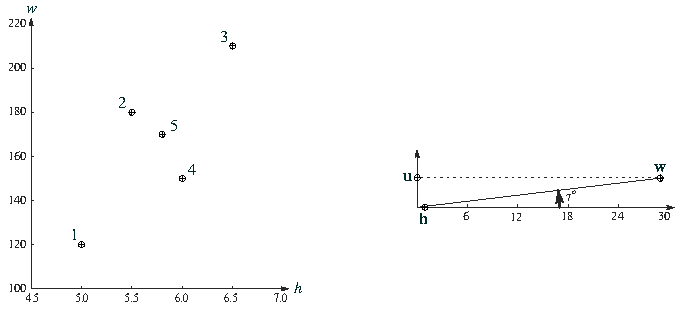
\includegraphics[scale=1.25]{./images/heightWeight.pdf}
\caption{(left) The height and weight coordinates for the five individuals in
the table.  The odd numbered points are nearly collinear to a line with a
slope of about $60$ while the even numbered points are more spread out.
(right)  The vector $\mathbf{h}$ points to the right in the horizontal 
direction while the vector $\mathbf{u}$ points in the upward vertical 
direction.  The length of $\mathbf{u}$ is about $3.5$ times the length of 
$\mathbf{h}$ and the length of $\mathbf{w}$ is about $8$ times the length of
$\mathbf{u}$.  The cosine similarity of $\mathbf{h}$ and $\mathbf{w}$ is about 
0.9925 and the angle between $\mathbf{h}$ and $\mathbf{w}$ is about $7^o$.} 
\label{twogeoms}
\end{figure}

   The other main way to think geometrically about the numbers in the table is 
to let the columns for the heights and weights be the coordinates for two 
points in $\real^5$.  Since this space has 5 dimensions we can not visualize 
these points directly but we do have the advantage in this case that there are 
only two points so they have to be contained within a 2 dimensional subspace
of $\real^5$.  We denote the vector of heights with:
\begin{equation*}
\mathbf{h} = (5.0,\, 5.5,\, 6.5,\, 6.0,\, 5.8)
\end{equation*}
and the vector of weights with:
\begin{equation*}
\mathbf{w} = (120,\, 180,\, 210,\, 150,\, 170)
\end{equation*}
For the purpose of visualzing the geometrical relationship between 
$\mathbf{h}$ and $\mathbf{w}$ we define another vector
\begin{equation*}
\mathbf{u} = (-24.8187,\, 20.6994,\, 21.7356,\, -23,7825,\, 2.0103)
\end{equation*}
It can be checked that to three digits:
\begin{equation*}
\mathbf{h} \bullet \mathbf{u} \approx 0 \quad \mbox{and} \quad
\mathbf{w} \approx 28.964 \, \mathbf{h} + \mathbf{u}
\end{equation*}
so that $\{ \mathbf{h}, \mathbf{u} \}$ is nearly orthogonal basis for the span
of $\{ \mathbf{h}, \mathbf{w} \}$.  The vector $\mathbf{w}$ is about $30$ 
times as long as the vector $\mathbf{h}$.  This is shown in the right panel of
figure \ref{twogeoms}.

% u is constructed to be orthogonal to h so we can see we are in a 2d subspace that contains h and w.  
% the heads of the vectors are shown with crosshairs
% h is pretty small so possibly change the data. 
% From one figure to another  we center, and notice the cosine similarity changes
The cosine similarity of the data gives us the cosine of the angle between the two points 
as measured from the origin of $\real^5$.

\begin{figure}[h]
\centering
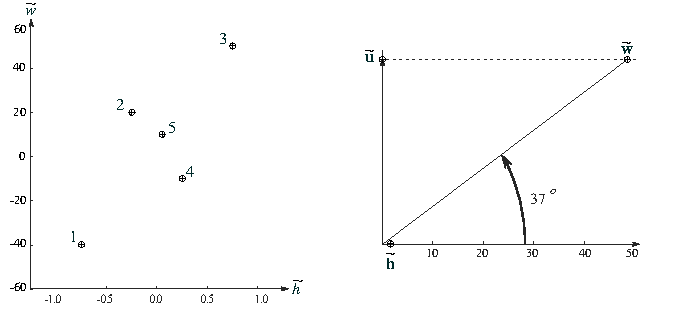
\includegraphics[scale=1.25]{./images/heightWeight2.pdf}
\caption{(left) The centered height and weight coordinates for the five 
individuals in the table.  The odd numbered points are again early collinear to 
a line with a slope of about $60$ while the even numbered points are more 
spread out.  (right)  The vector $\widetilde{\mathbf{h}}$ points to the right 
in the horizontal direction while the vector $\widetilde{\mathbf{u}}$ points in 
the upward vertical direction.  The length of $\widetilde{\mathbf{u}}$ is about 
$36$ times the length of $\widetilde{\mathbf{h}}$ and the length of 
$\widetilde{\mathbf{w}}$ is about $1.7$ times the length of 
$\widetilde{\mathbf{u}}$.  The cosine similarity of $\widetilde{\mathbf{h}}$ 
and $\widetilde{\mathbf{w}}$ is about 0.800 and the angle between 
$\widetilde{\mathbf{h}}$ and $\widetilde{\mathbf{w}}$ is about $37^o$.} 
\label{twogeoms2}
\end{figure}
